\section{Background and Motivation}

\subsection{Introduction}
Cancer is, today, the second leading cause of death in the world, only behind cardiovascular diseases.\\  %TODO CITE
It is one of the leading causes of mortality worldwide, with approximately 14 million new cases in 2012. %TODO  "http://www.who.int/mediacentre/factsheets/fs297/en/ World Health Organization. February 2018. Retrieved 19 April 2018.
It is defined as a disease that has an abnormal cell growth with the potential to spread into other parts of the body.%TODO https://www.cancer.gov/about-cancer/understanding/what-is-cancer
Contrary to normal cells, cancer cells are often invasive, and it will spread if not treated. 
In contrast to many other diseases, cancer does not start from a foreign entity (such as a bacteria or virus), but it is often from a malfunctioning cell that starts dividing rapidly. 
This cell division can happen when a cell is damaged, by for instance by radiation or other factors specific proteins, or other chemicals. The result is that the cell either has damage in the DNA which contributes to abnormal cell division or the cell division itself malfunctions. In both cases the damage causes the cell to divide uncontrollably. 
Cancer can in some cases form without any external forces. The cell division is not always perfect, and dysfunctional cells might start a rapid division after being born. In most cases, this is not a problem, as most cells self destruct when they cannot operate\todo{cite}. 

Another factor that increases the risk of cancer is age. As we grow older, our body gets more prone to defective cell division and for each imperfect division the chance of getting cancerous cells increases.  
Our own body is designed to detect and remove cells that are prone to divide uncontrollably. Unfortunately, this system is not perfect, and the immune system can in some cases overlook cells that are cancerous.
In either external or internal cases, cancer is by definition this uncontrollable multiplication.




\textbf{Statistics on cancer}\\
Since cancer is, in practice, just a cell division error, it has the opportunity to hit anyone, at any age. Because of this, it is a heavily reseached area, both in Norway, and the rest of the world.
In 200X we spent 22Y million dollars worldwide on cancer research. 
Despite being such a researched area, it is still one of the top causes of human death. 
Some types of cancer, like \todo{} cancer, is one of the simpler forms of cancer to treat, and at this point, those kind of cancers are non-fatal. 
\textit{The most common types of cancer in males are lung cancer, prostate cancer, colorectal cancer and stomach cancer.\cite{stewart2014world}}
    
\textbf{colorectal cancer}\\
Humans can get cancer in every major organ, but some types of cancer are more common than others.    
For instance cancer in the gastrointestinal tract (GI) is one of the more common places to get cancer. Colorectal cancer is just behind x as the most common cancer for men, and it has a mortality rate of x in the first y years. %TODO CITE 
We often call this 5-year survival rate for z. Z is the standard way to measure the life expectancy of a patient diagnosed with cancer. 
    

\textbf{polyps}\\
Colorectal cancer often starts in polyps. 
Polyps are, polyps do.
    
\textbf{preventative matters and early detection}\\
    \textit{-colonoscopy\\ 
        -mri\\
        -pillcam\\}
    As stated, the best way to fight cancer is to detect and remove it early, or in some cases, remove areas with a high chance of getting cancer.
    We classify cancer into four stages\todo{cite}, and the stage the patient is in often determines the chance he/she has for survival. 
    In general, the earlier doctors detect the cancerous parts, the more likely it is that the patient will survive. 
    Moreover, as mentioned above, colorectal cancer often starts in these polyps. A crucial stage to prevent cancer lies in the 
    early removal of there polyps.
    Reports show x about this %TODO find Reports.
    
    \begin{figure}
        \centering
        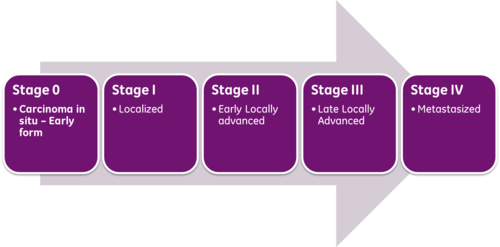
\includegraphics[scale=0.05]{introduction/figures/Cancer_stages.png}
        \caption{Stages of cancer from wikipedia} 
    \end{figure}

        
    Because of this the ability to find, and remove colorectal polyps is excellent for preventing cancer in the GI tract. 
    
    
    \vspace{10px}
    \textbf{colonoscopy/Ontonoscopy}
    In the most common way to look for polyps in the GI tract is to use a medical team, and perform a colonoscopy or Ontonoscopy
Colonoscopy is performed with a camera-stick that is inserted into the GI tract through the patients' anus.\\
    Onoskopy is the same procedure; only the camera is inserted orally. \\
    
    \textbf{Advantages}
      \begin{itemize}
        \item Accuracy: The use of a camera controlled by the doctor gives him/her the opportunity to stop at any anomalies.
        \item Quick results: Since the doctor is doing the procedure the result is given live.
      \end{itemize}

    \vspace{5px}
    \textbf{Disadvantages}
      \begin{itemize}
        \item Expensive: The cost of the doctor and the nurses needed is often high, especially on a routine check.
        \item Invasion of privacy: Getting a Colonoscopy or Onoskopy is a %TODO
      \end{itemize}
    
    \vspace{10px}
    \textbf{MRI}
    MRI (Maggnetic stuff) is the act of taking pictures blabla blabla\\
    MRI (Maggnetic stuff) is the act of taking pictures blabla blabla\\
    MRI (Maggnetic stuff) is the act of taking pictures blabla blabla\\
    %TODO MRI VS CT
    \textbf{Advantages}
      \begin{itemize}
        \item This is why MRI is good %TODO.
        \item This is why MRI is good %TODO.
      \end{itemize}

    \vspace{5px}
    \textbf{Disadvantages}
      \begin{itemize}
        \item This is why MRI is bad %TODO.
        \item This is why MRI is bad %TODO.
      \end{itemize}
    \vspace{10px}
    \textbf{pillcam}
    In the last 3-4 years, there have been testing and development on the pillcam project EIR. Machine learning has, through many of the earlier projects, got the detection rate for the polyps up to x\% %TODO Cite.
    
    \textbf{Advantages}
      \begin{itemize}
        \item This is why pillcam is good %TODO.
        \item This is why pillcam is good %TODO.
      \end{itemize}

    \vspace{5px}
    \textbf{Disadvantages}
      \begin{itemize}
        \item This is why cam is bad %TODO.
        \item This is why pillcam is bad %TODO.
      \end{itemize}
 
    
    
    \vspace{10px}

\textbf{Simulas contribution to the pillcam project}\\
    Simulas EIR
        

        
    * CAD ACD (computer-aided diagnosis, Automated computer diagnosis)

    \vspace{10px}
    
    
\section{Problem definition}
\section{Research Method}
\section{Main contriburors and related work}
\section{Outline}
